% SpaceCHI 2026 position paper / camera-ready manuscript.
% The supplied Springer proceedings template is used without class modification.
\documentclass[runningheads]{llncs}

\usepackage[T1]{fontenc}
\usepackage{graphicx}
\usepackage{float}
\usepackage{booktabs}
\usepackage{array}
\usepackage{amsmath}
\usepackage{url}
\usepackage{xcolor}
\setlength{\emergencystretch}{3em}
\pagecolor{white}

\begin{document}

\title{Superman Suit: A Photovoltaic Neuromuscular Safety Net for Off-World Habitats}
\titlerunning{Superman Suit: A Neuromuscular Safety Net}

\author{Taechasith Kangkhuntod\inst{1} \and Nantita Damrongpanawan\inst{2}}
\authorrunning{T. Kangkhuntod and N. Damrongpanawan}
\institute{University of the Thai Chamber of Commerce, Bangkok, Thailand
\and Bangkok University, Bangkok, Thailand}

\maketitle

% Figure 1 is intentionally before the abstract.
\begin{figure}[H]
\centering
\IfFileExists{figures/fig1_suit_design.pdf}{%
  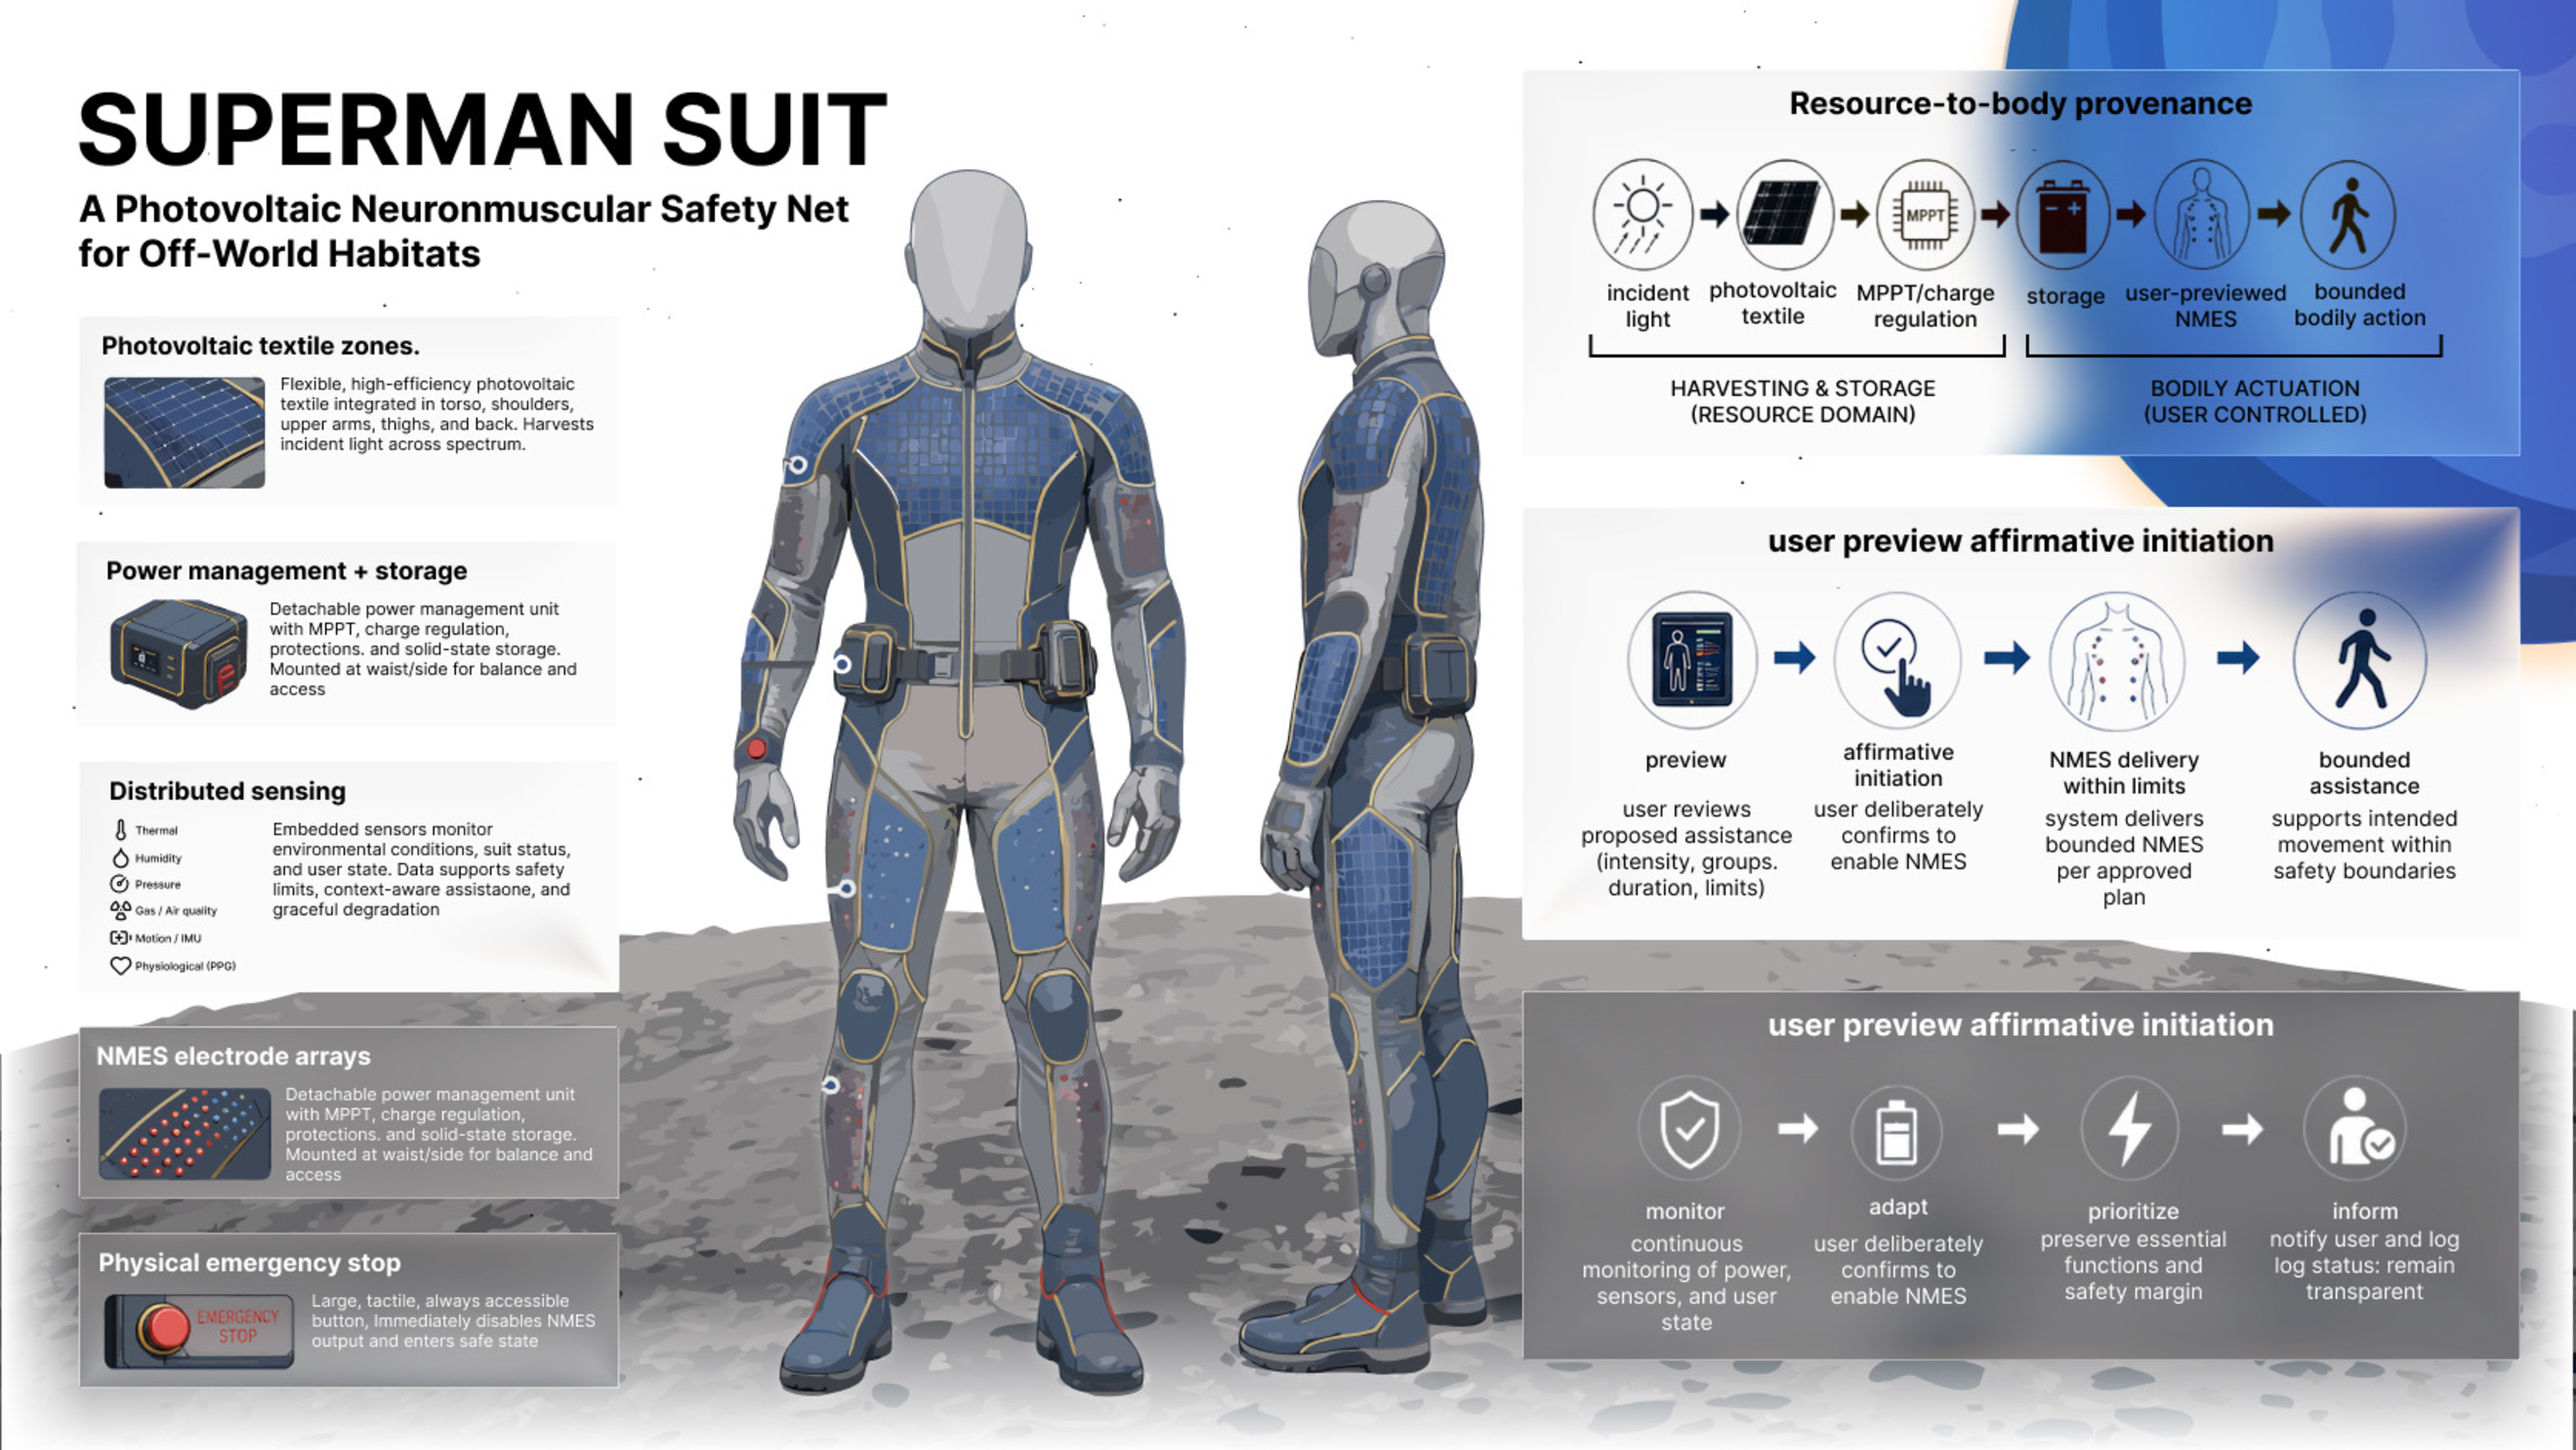
\includegraphics[width=0.94\textwidth]{figures/fig1_suit_design.pdf}%
}{%
  \fbox{\parbox[c][0.22\textheight][c]{0.90\textwidth}{\centering
  \textit{Figure 1 placeholder: insert the annotated Superman Suit design here.}\\[3pt]
  \small Photovoltaic textile; storage and power electronics; distributed sensing;\\
  \small user-controlled neuromuscular stimulation; local emergency stop.}}
}
\caption{Illustrative overview of the proposed Superman Suit as a resource-to-body system. The guide identifies the garment, photovoltaic zones, storage and control module, electrode locations, sensing, data/energy provenance, and wearer-facing safety controls.}
\label{fig:suit-overview}
\end{figure}

\begin{abstract}
Future off-world habitats may treat the human body as another load on centralized systems for power, exercise, and health maintenance. This position paper argues that Space HCI should also investigate garments as distributed physiological infrastructure: body-proximate systems that harvest local resources, make scarcity legible, and preserve bounded care when centralized infrastructure is interrupted. We develop this position through the \emph{Superman Suit}, a conceptual photovoltaic garment that stores harvested light energy and allocates it to user-controlled neuromuscular electrical stimulation (NMES) when ordinary exercise is temporarily unavailable. Its bounded design target is activation continuity: retaining the capability to complete one preauthorized, user-initiated lower-limb NMES session during a 24--72-hour outage, not reproducing exercise or claiming protection from deconditioning. The suit is not proposed as an exercise replacement, clinical device, or flight-qualified system. Instead, it is a theory-bearing artifact for examining environmental intermittency, resource provenance, uncertainty, bodily automation, and crew agency. Following design science and Research through Design, we combine literature grounding, an annotated system model, failure-first interaction scenarios, and a bounded computational energy probe. Rather than treating exact simulated probabilities as predictions, the probe identifies transitions among autonomous-candidate, conditional, assisted, and unavailable states and the assumptions that drive those transitions. We contribute the strong concept of a \emph{metabolic safety net}, seven design propositions, and a staged research agenda that can challenge or falsify the proposal.

\keywords{Space HCI \and wearable technology \and neuromuscular electrical stimulation \and photovoltaic textiles \and design science \and Research through Design \and human autonomy}
\end{abstract}

\section{Introduction}

Long-duration spaceflight makes bodily maintenance an infrastructure problem. Exercise countermeasures, clinical oversight, power, data, and maintenance are coupled to a habitat that is itself exposed to interruptions, constrained mass, and operational uncertainty. NASA's evidence review identifies reduced muscle mass, strength, endurance, and aerobic capacity as performance risks and treats exercise as a central countermeasure [1]. The practical burden is not only the exercise dose: setup, stowage, hygiene, scheduling, and equipment maintenance consume scarce crew time and habitat resources. Reports of cable wear in the International Space Station countermeasures system illustrate how a mundane component can interrupt an otherwise established capability [14,15].

This paper asks what Space HCI can contribute when a health garment is designed as infrastructure rather than as personal electronics. We propose the \emph{Superman Suit}: a conceptual garment that harvests light through photovoltaic textile surfaces, stores a bounded energy reserve, and uses that reserve to support user-controlled NMES when a primary exercise capability is temporarily unavailable. The name is a memorable metaphor for a protective safety net, not a claim of superhuman enhancement.

We bind the proposal to short, recoverable interruptions rather than an indefinite failure: for example, 24--72 hours while a treadmill or resistive device is inspected or repaired, a scheduled exercise period missed during temporary rover or safe-haven isolation, or a short habitat power-allocation interruption. The target capability is to deliver one session already authorized by a clinician, with measurable electrical delivery and an immediate local stop. Whether that session produces adequate evoked force or any protective physiological effect remains an empirical question. Medical contraindication, loss of clinical authorization, long-duration exercise loss, or habitat emergency makes the suit unavailable rather than expanding its role.

Our position is deliberately narrower than a product claim. The suit is not an exercise replacement, a prescription for stimulation parameters, a clinical intervention, or a flight-ready system. It is a theory-bearing artifact through which to examine how environmental resources become bodily action. The central claim is:

\begin{quote}
Space HCI should treat off-world health garments as distributed, resource-aware physiological infrastructure: systems that sense local resource availability, preserve a bounded reserve, explain how that reserve is allocated to the body, and maintain limited care during infrastructural interruption.
\end{quote}

The paper makes three contributions. First, it introduces the \emph{metabolic safety net}, a strong concept for limited physiological continuity during failure. Second, it instantiates that concept in an annotated suit architecture and interaction model that foreground resource provenance, uncertainty, consent, and refusal. Third, it contributes a design-science research agenda, including design propositions, failure conditions, and a computational probe that disciplines material plausibility without being mistaken for human validation.

\section{Why This Is a Space HCI Problem}

\subsection{From exercise equipment to distributed infrastructure}

Human spaceflight countermeasures are usually framed as dedicated equipment, scheduled procedures, or clinical protocols. This framing is useful for accountability, but it can obscure the relationship between environmental resources, maintenance work, bodily agency, and system failure. A garment makes these relationships intimate: energy is gathered on the body, stored near the body, and ultimately converted into a bodily stimulus. The design therefore has to communicate not just status, but provenance: where the energy came from, how much is available, how uncertain that estimate is, and what bodily action it can support.

The proposal builds on three established observations. First, exercise remains the benchmark countermeasure for deconditioning in spaceflight [1]. Second, NMES can evoke muscle contraction and has been investigated in spaceflight and bed-rest contexts, but its delivered current, monitoring, and resultant force require explicit measurement [3,4]. Third, photovoltaic textiles and flexible solar materials demonstrate a direction for body-conformal harvesting, while their practical performance depends strongly on geometry, illumination, packaging, durability, comfort, and integration [6,7,21]. These observations support a research opportunity, not a deployment conclusion.

Existing work already demonstrates the components separately: an EMS garment has been used for weightless squats [2], photovoltaic textiles harvest energy [6,7], and smart textiles combine sensing, power, and interaction functions [21]. The proposed difference is therefore not a novel electrode or photovoltaic material. It is the HCI coupling of energy provenance and uncertainty to a user-governed bodily capability during infrastructure failure.

\subsection{Why intermittency matters}

The lunar south pole combines long-duration illumination geometry, shadow, thermal extremes, and dust concerns [8]. Mars adds atmospheric dust and regional or global storms that can attenuate sunlight [9]. Habitats also create their own interruptions: a solar-facing window may be unavailable, an external array may be isolated, or an exercise device may be reserved, degraded, or under maintenance. A resource-aware garment must therefore have explicit states for autonomous support, hybrid support, and unavailable support. A design that silently assumes continuous light converts a contingency system into a hidden single point of failure.

\subsection{HCI stakes: agency, trust, and bodily governance}

The suit would not merely display a battery percentage. It would negotiate a boundary between crew autonomy and automated resource allocation. A system that actuates the body must be previewable, interruptible, and intelligible. NASA's human-system standard provides a relevant human-factors baseline for crew interfaces [10], while the safety and essential-performance requirements for nerve and muscle stimulators provide a reminder that a wearable concept cannot bypass medical-device constraints [13]. These requirements motivate the design concepts of resource-to-body legibility, bounded bodily automation, and safe scarcity developed below.

\section{Design-Science Position}

\subsection{Design science and Research through Design}

Design science develops knowledge by constructing and evaluating artifacts that extend human or organizational capabilities [17]. Research through Design (RtD) uses the act of making a designed artifact to produce knowledge that is relevant, inventive, and extensible beyond the artifact itself [18]. RtD knowledge may be provisional and contingent, but it remains rigorous when the artifact, design reasoning, annotations, and limits are made visible [19]. Strong concepts provide an intermediate level of abstraction: more transferable than a single product, but close enough to interaction to guide design decisions [20].

The Superman Suit is therefore treated as a \emph{theory-bearing artifact}. It is not evidence that a photovoltaic NMES suit preserves muscle in space. Its role is to make a set of relationships discussable and falsifiable:

\begin{itemize}
\item environmental energy becomes a bodily reserve;
\item the reserve is intermittent, uncertain, and physically situated;
\item the user must understand and authorize bodily actuation; and
\item a failure mode should degrade capability visibly rather than increase risk.
\end{itemize}

The design-science cycle has three linked parts. The relevance cycle frames exercise interruption, maintenance burden, resource scarcity, and crew autonomy. The rigor cycle draws on space-health evidence, NMES limitations, photovoltaic textiles, human factors, and medical-device safety. The design cycle constructs, annotates, stress-tests, and revises the suit concept. The output is intermediate-level design knowledge rather than a validated biomedical result.

\subsection{The metabolic safety net}

The central concept is a \emph{metabolic safety net}: a secondary, distributed system that maintains a bounded physiological-care function when a primary countermeasure is interrupted. The word \emph{bounded} is essential. Here the target is \emph{activation continuity}: the capacity to complete one preauthorized lower-limb NMES session during a 24--72-hour interruption while recording delivered output, contact quality, and stop events. Future evaluation must measure evoked force or torque; current delivery alone is not a physiological outcome. The safety net does not reproduce the cardiovascular, skeletal, sensorimotor, or psychosocial benefits of a treadmill, cycle ergometer, or resistive exercise device. ``Metabolic'' names continuity of body-maintenance infrastructure, not a demonstrated whole-body metabolic effect.

This concept produces four design commitments. First, contingency takes priority over substitution: the system is judged by continuity during interruption, not equivalence during nominal operation. Second, resource provenance precedes actuation: the wearer sees how an environmental resource is becoming bodily action. Third, scarcity is safe: declining energy reduces or postpones capability and never justifies exceeding an approved stimulation envelope. Fourth, bodily sovereignty is explicit: sessions require preview, affirmative initiation, and an immediate local stop.

\subsection{Design propositions}

The following propositions are intentionally contestable. They provide intermediate-level claims that can organize future design and empirical work.

\begin{description}
\item[DP1 -- Distributed continuity.] Off-world health systems should preserve a minimum distributed care capability so bodily maintenance does not disappear completely when centralized equipment fails.
\item[DP2 -- Provenance before actuation.] A resource-aware wearable should disclose energy origin, available quantity, uncertainty, and the bodily action that the reserve can support before actuation.
\item[DP3 -- Bodily sovereignty.] Any system that actuates the body should require preview, affirmative initiation, immediate local stop, and intelligible post-action accounting.
\item[DP4 -- Safe scarcity.] Energy scarcity should reduce, defer, or cancel functionality; it must never justify exceeding an approved stimulation or discomfort envelope.
\item[DP5 -- Countermeasure plurality.] A physiological wearable should be one layer in a portfolio of countermeasures, not a totalizing replacement for exercise, clinical care, or habitat infrastructure.
\item[DP6 -- Failure-first evaluation.] Resource-aware physiological systems should be evaluated through outages, uncertainty, sensor disagreement, and user refusal, not only through nominal operation.
\item[DP7 -- Evidence-bound speculation.] Speculative artifacts become scientifically useful when each claim is labeled as established evidence, design inference, computational result, or future empirical question.
\end{description}

\section{The Superman Suit as a Design Instantiation}

\subsection{System architecture}

The proposed garment is a layered system rather than a single fabric. A photovoltaic textile layer collects incident light over torso and limb surfaces. A power-management layer performs maximum-power-point tracking, charge regulation, and electrical isolation. A storage layer holds a reserve sized for an explicitly bounded session. A sensing layer estimates illumination, garment contact, skin or electrode impedance, motion, temperature, and electrical output. A stimulation layer delivers a charge-balanced, clinician-defined NMES waveform through localized electrodes. A wearer-facing interface communicates provenance, reserve, uncertainty, session preview, and stop state. These layers are conceptual requirements, not a completed bill of materials.

The energy path is intentionally visible:

\begin{equation}
E_{\mathrm{light}} \rightarrow E_{\mathrm{PV}} \rightarrow E_{\mathrm{stored}} \rightarrow E_{\mathrm{NMES}} \rightarrow \text{bounded bodily action}.
\end{equation}

At every transition, the system should expose losses and uncertainty. A high battery state cannot be presented as available stimulation energy if electrode impedance, converter overhead, thermal constraints, or session policy prevent delivery.

Integration is justified only where coupling creates interaction value. Co-locating harvesting, reserve estimation, contact sensing, stimulation state, and the physical stop lets one interface explain how much locally harvested energy can support which authorized bodily action, and lets a single fail-safe state disable actuation. It may also reduce repeated positioning and loose interconnects. However, integration adds mass, heat, fit, laundering, repair, and certification burdens. The theory therefore requires an integrated resource-to-body account and safety controller, not that every component be permanently sewn into one fabric. A photovoltaic overshirt plus removable storage and a separately certified NMES underlayer is a valid, and possibly preferable, implementation baseline.

The figures make four theory-relevant placement choices: photovoltaic zones occupy outward-facing surfaces; electrodes align with candidate large lower-limb muscle regions; power hardware is isolated and removable; and a physical stop remains locally reachable. The exact panel shapes, electrode count and sites, sensor distribution, and stop location are illustrative rather than derived or clinically approved. Their purpose is to expose dependencies for later ergonomic, electrical, and clinical testing.

\subsection{Interaction states}

The garment has five user-visible states:

\begin{enumerate}
\item \textbf{Harvesting:} light and charge rate are displayed, with the active harvesting surface and environmental uncertainty.
\item \textbf{Reserve:} stored energy is reported as usable session time under the selected protocol, not only as a percentage.
\item \textbf{Preview:} the wearer or an authorized clinician sees the intended muscles, duration, waveform envelope, expected discomfort, and energy cost.
\item \textbf{Active:} the session shows delivered output, contact quality, stop affordance, and remaining reserve.
\item \textbf{Degraded or unavailable:} the system explains why a session is shortened, deferred, or blocked and offers non-actuating alternatives.
\end{enumerate}

The design forbids autonomous background stimulation. A scheduler may recommend a session when resource and mission conditions are favorable, but the session must still require affirmative initiation. The emergency stop is physical, locally reachable, and independent of the display or network. If sensing disagrees or the wearer refuses, the safe outcome is to stop or defer.

\subsection{Illustrative suit design}

Figure~\ref{fig:suit-detail} uses the same suit architecture and visual language as Figure~\ref{fig:suit-overview} while separating photovoltaic and power layers from bodily sensing and actuation layers. It annotates the photovoltaic zones, removable electronics, illustrative electrode and sensor regions, charging and data paths, and the physical emergency stop. It also shows what the wearer can see before and during a session. The important distinction is between the \emph{resource layer} (harvesting, storage, and uncertainty) and the \emph{bodily layer} (sensing, stimulation, and user control), not the unvalidated geometry of a particular panel.

\begin{figure}[H]
\centering
\IfFileExists{figures/fig2_suit_design_detail.pdf}{%
  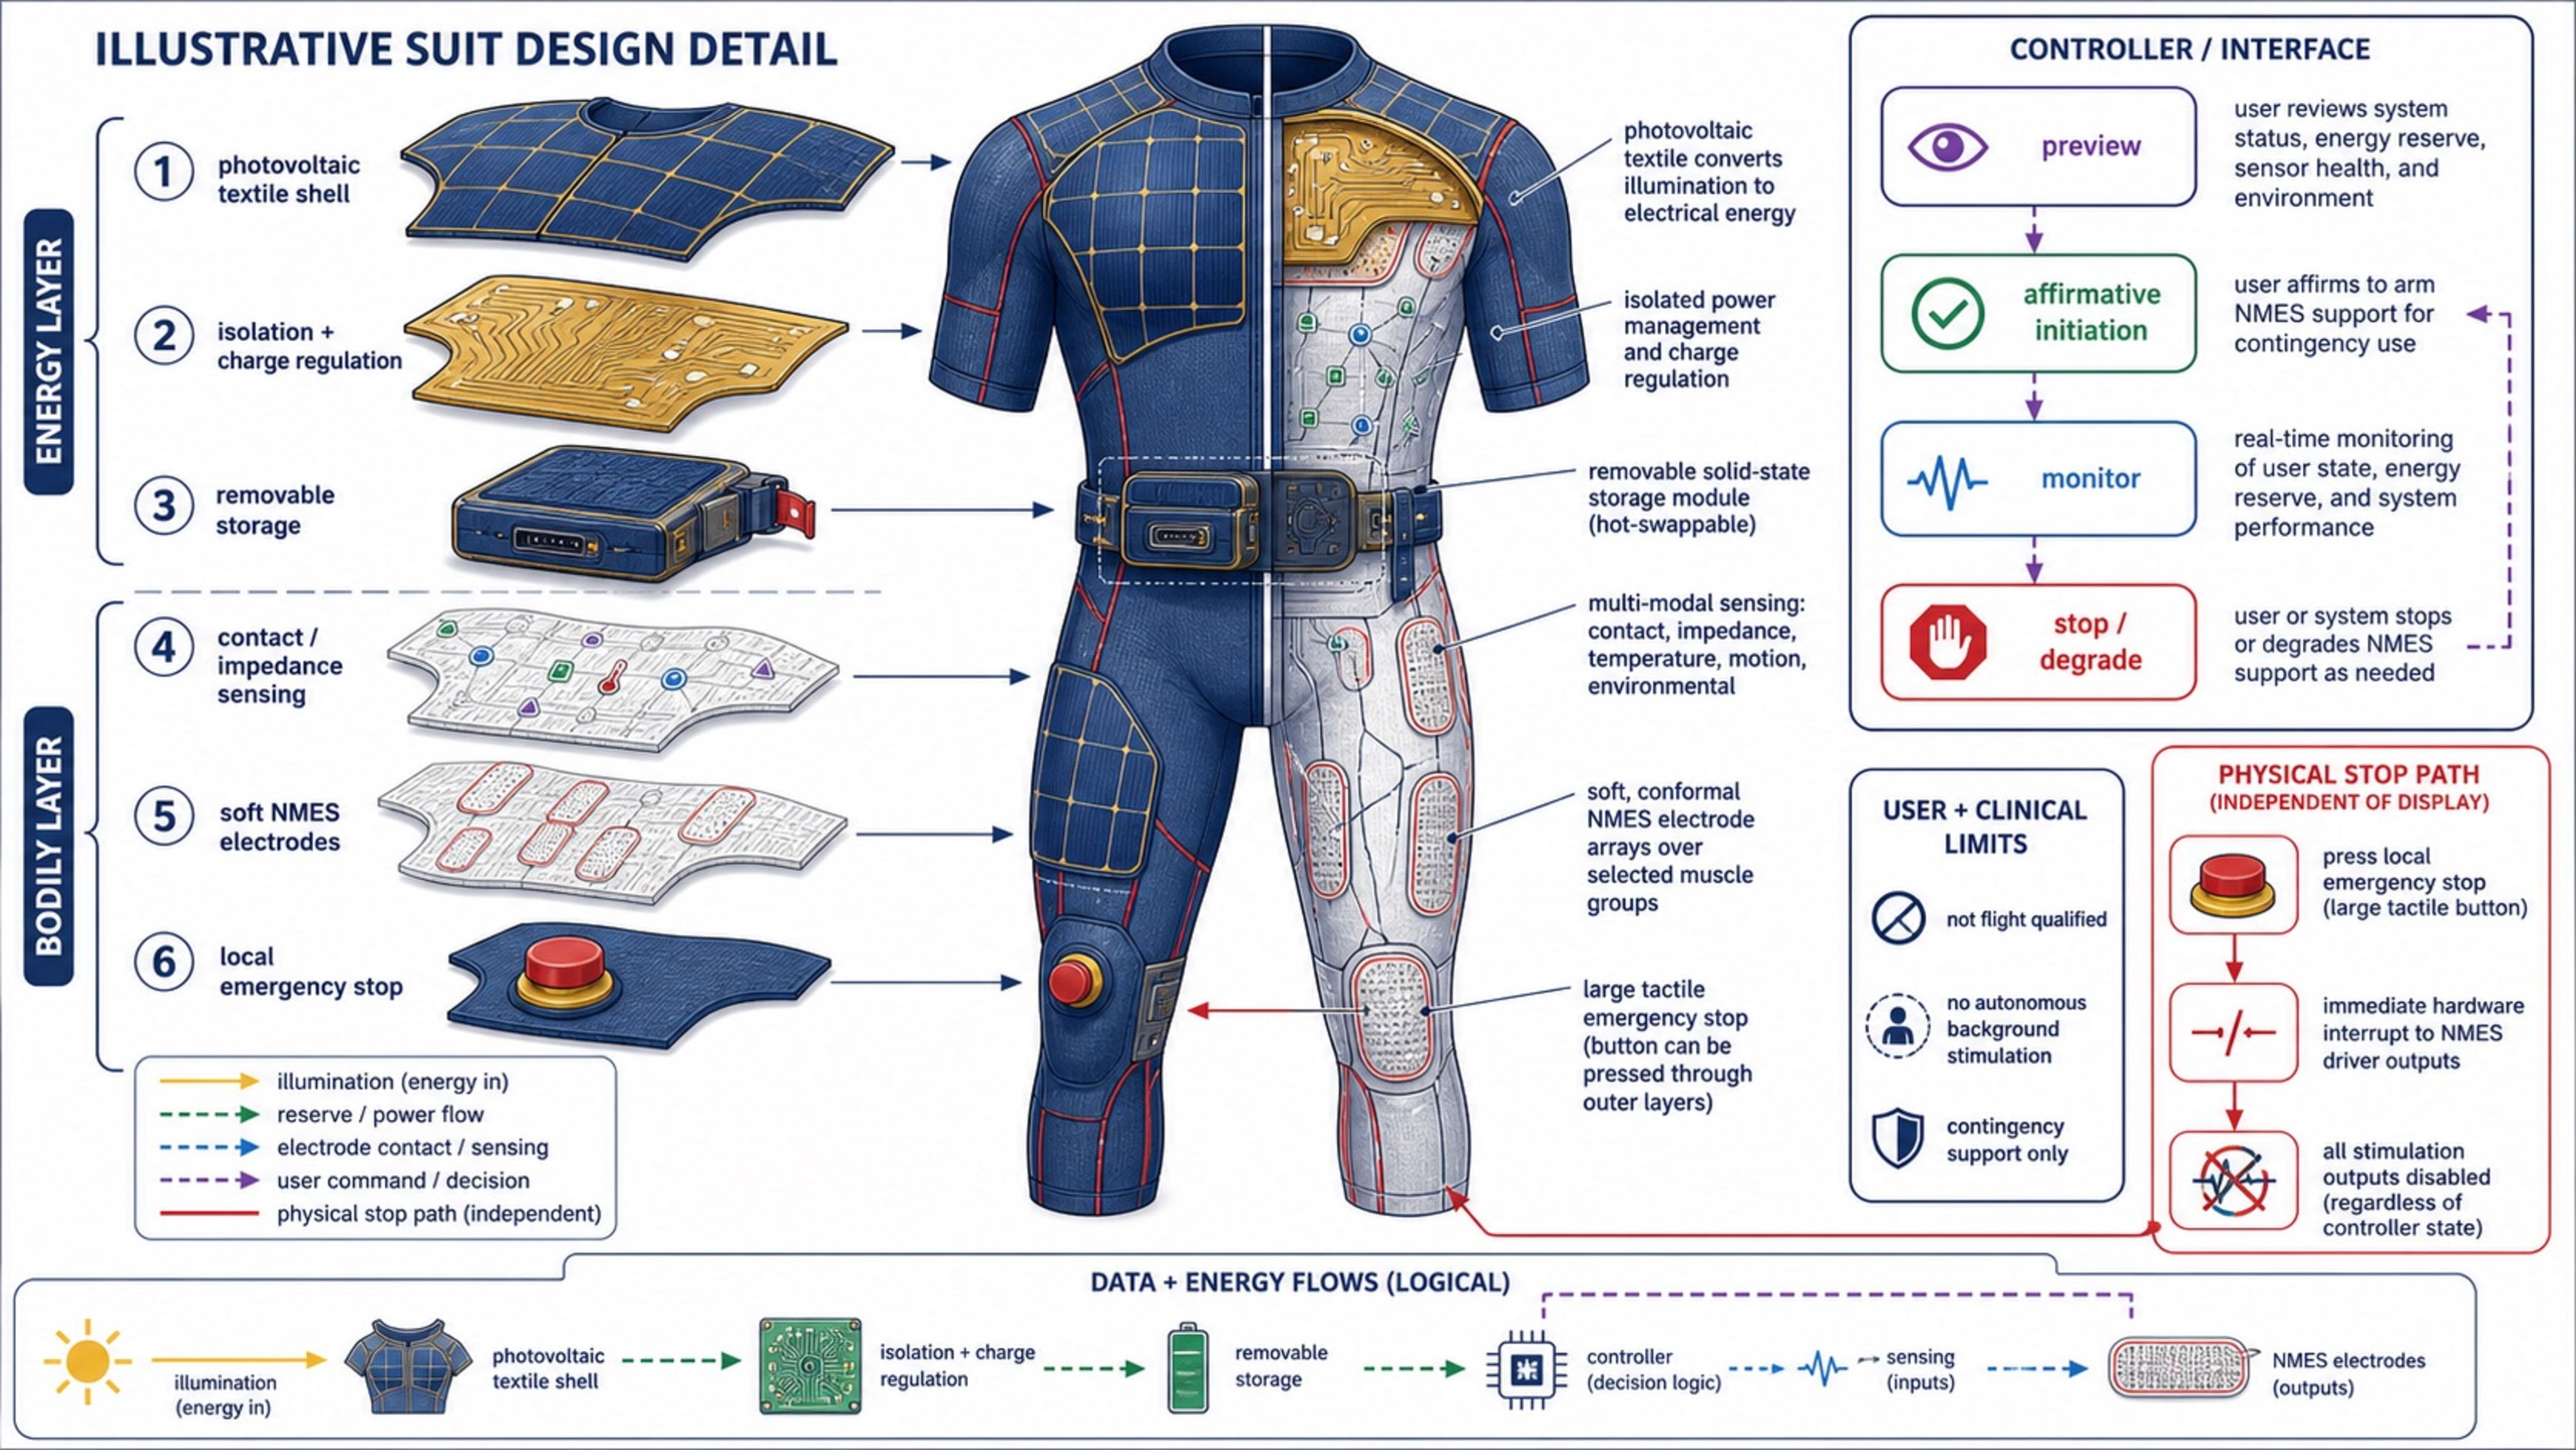
\includegraphics[width=0.94\textwidth]{figures/fig2_suit_design_detail.pdf}%
}{%
  \fbox{\parbox[c][0.20\textheight][c]{0.90\textwidth}{\centering
  \textit{Figure 2 placeholder: annotated suit detail for the design illustration section.}\\[3pt]
  \small Mark PV zones, storage/controller, electrodes, sensors, emergency stop,\\
  \small and the wearer-facing resource-to-body information flow.}}
}
\caption{Illustrative suit-design detail, matched to the garment in Fig.~\ref{fig:suit-overview}. Numbered targets map the exploded layers to specific suit components; vector leaders terminate on the photovoltaic shell, controller, storage, sensor nodes, and electrodes. Logical arrows show information and energy direction rather than physical wire routing. Exact component placement is not clinically or ergonomically validated.}
\label{fig:suit-detail}
\end{figure}

\subsection{Mission-life integration and acceptance}

The default use pattern is session-specific rather than continuous wear. A crew member retrieves the garment after an eligible interruption, connects charged removable modules, checks fit and contact, reviews source, reserve, uncertainty, muscle regions, duration, and limits, and then either initiates or refuses the session. Afterwards, the system reports delivered output and stop history before the soft layer is cleaned and the electronics are inspected and stowed. Harvesting may occur while the unworn garment is positioned near a protected illuminated surface; the concept does not imply use during extravehicular activity or underneath a pressure suit.

No astronaut has yet evaluated this workflow, so these are user-need hypotheses, not astronaut requirements. Body-worn-sensor research emphasizes compactness, embedding, simple operation and maintenance, and minimal disruption to ordinary behavior [22]. Participatory work with astronauts, flight surgeons, exercise specialists, and maintainers should therefore test donning time, fit across bodies, heat and moisture, skin tolerance, mobility, cable snagging, privacy, social visibility, alarm burden, cleaning, repair, and whether provenance displays aid decisions or merely add workload. Acceptance is a gate: a technically feasible garment that disrupts sleep, work, hygiene, or bodily autonomy fails as a safety net.

\section{Failure-First Scenarios and Safety Boundaries}

The concept is evaluated by the situations in which its assumptions fail. Table~\ref{tab:scenarios} summarizes five resource scenarios used to structure the design probe and the interaction requirements. These are charging and energy-accounting contexts, not evidence that the garment is suitable for every named environment.

\begin{table}[ht]
\caption{Failure-first scenarios for the Superman Suit.}
\label{tab:scenarios}
\centering
\small
\begin{tabular}{p{0.20\textwidth}p{0.32\textwidth}p{0.34\textwidth}}
\toprule
Scenario & Resource condition & Required system response \\
\midrule
Indoor habitat & Low-to-moderate, variable illumination & Show conditional support; recommend external charging or primary exercise. \\
Window-filtered habitat & Stronger but filtered illumination & Report conversion loss and usable charge duration. \\
Lunar deployment & High incident light but thermal, dust, and geometry constraints & Separate local harvest from mission-wide power and maintenance assumptions. \\
Mars clear deployment & Strong outdoor light with dust uncertainty & Make environmental confidence and predicted reserve visible. \\
Light interruption & Zero or near-zero harvest during a session & Stop, shorten, or switch to stored-reserve mode without increasing stimulation risk. \\
\bottomrule
\end{tabular}
\end{table}

The safety boundary is not an optimization target. The control policy is lexicographic: (1) stop on unsafe contact, impedance, temperature, or command disagreement; (2) enforce the clinician-defined stimulation envelope; (3) preserve a minimum reserve for emergency and diagnostic operation; (4) optimize session timing and harvested-energy use. An energy-aware controller may choose a smaller session, but it may never choose a higher current merely because more physiological work is desired.

\section{A Bounded Computational Design Probe}

\subsection{Purpose and scope}

The computational study is an evaluative design probe. It asks whether the proposed resource-to-body loop is materially plausible under declared assumptions and which assumptions dominate the result. It does not estimate muscle preservation, discomfort, long-term efficacy, clinical safety, or mission readiness. No human or animal data were collected.

\subsection{Model}

We sampled an illustrative energy model with triangular distributions for incident irradiance, active area, textile conversion efficiency, optical and packaging losses, MPPT and storage efficiency, electronics overhead, and stimulation demand. For each draw, harvested electrical energy was estimated as

\begin{equation}
E_{\mathrm{harvest}}=G A_{\mathrm{PV}}\eta_{\mathrm{PV}}\tau\eta_{\mathrm{MPPT}}\eta_{\mathrm{store}}t_{\mathrm{charge}},
\end{equation}

where $G$ is irradiance, $A_{\mathrm{PV}}$ is active area, $\eta_{\mathrm{PV}}$ is conversion efficiency, $\tau$ captures optical and packaging transmission, and $t_{\mathrm{charge}}$ is usable charging time. The session demand includes a simplified pulsed electrode load and a fixed electronics overhead:

\begin{equation}
E_{\mathrm{demand}}=t_{\mathrm{session}}(P_{\mathrm{electrode}}+P_{\mathrm{overhead}}).
\end{equation}

The energy adequacy ratio is $\mathrm{EAR}=E_{\mathrm{harvest}}/E_{\mathrm{demand}}$. A draw was counted as a preliminary energy-support case when $\mathrm{EAR}\geq1.20$ and the estimated output voltage remained below a declared compliance-envelope value. These thresholds are screening rules for the model, not medical or engineering standards.

\subsection{Scenarios, protocols, and reproducibility}

The probe crossed five scenarios with three candidate protocols and generated 50,000 draws per scenario--protocol pair (750,000 observations total). The scenarios were indoor habitat, window-filtered habitat, lunar deployed sunlight, Mars clear deployed sunlight, and light interruption. The protocols were a 30-minute two-channel bridge-light session, a three-by-30-minute anchored session, and a 45-minute four-channel multichannel screen. These names identify load profiles in the model; they do not prescribe a stimulation regimen. For discussion, \emph{autonomous-candidate} means that the declared energy screen was robust without external energy; \emph{conditional} means that the classification changed within plausible inputs; \emph{assisted} requires a precharged or external reserve; and \emph{unavailable} means that the modeled session should be blocked. None is a clinical-readiness label.

The run used a fixed seed (20260718), standard-library Python, versioned assumptions, boundary-case tests, and a SHA-256 manifest. An initial post-run audit found a defect in a unit-name checker; the checker was corrected without changing model equations or numeric outputs, and the final verification passed 17 of 17 tests. This audit trail is part of the result because evidence-bound speculation requires visible correction rather than silent cleanup.

\subsection{Results}

Table~\ref{tab:probe} foregrounds state transitions and sensitivity rather than precise probabilities. The full distributions, exact model-internal probabilities, boundary cases, assumptions, and code are supplied in the accompanying project directory.

\begin{table}[ht]
\caption{State transitions from the illustrative computational probe. EAR values are model outputs, not measured performance; exact success probabilities are retained only in the supplement.}
\label{tab:probe}
\centering
\scriptsize
\begin{tabular}{>{\raggedright\arraybackslash}p{0.19\textwidth}>{\raggedright\arraybackslash}p{0.22\textwidth}r@{\hspace{0.8em}}>{\raggedright\arraybackslash}p{0.27\textwidth}}
\toprule
Scenario & State & Median EAR & Interpretation \\
\midrule
Indoor habitat & Conditional $\rightarrow$ assisted & 0.626--1.887 & Irradiance and overhead can change the state. \\
Window-filtered & Autonomy candidate & 8.818--26.639 & Depends on usable exposure and filtering. \\
Lunar deployed & Autonomy candidate & 29.666--88.643 & Duration dominates; thermal and dust effects are omitted. \\
Mars clear deployed & Autonomy candidate & 12.117--36.609 & Duration is decisive; storms are outside this case. \\
Light interruption & Assisted $\rightarrow$ unavailable & 0.095--0.287 & No current harvest; actuation depends on prior reserve. \\
\bottomrule
\end{tabular}
\end{table}

Across all 15 scenario--protocol pairs, 9 entered the autonomous-candidate state, 1 was conditional and assumption-sensitive, 4 required an assisted framing, and 1 was unavailable. The transition pattern is the substantive result: deployed or strongly illuminated charging was robust under the declared assumptions, indoor operation moved between conditional and assisted, and interrupted-light operation moved between assisted and unavailable. Irradiance and charge duration were the strongest positive sensitivity drivers; electronics overhead was a recurring negative driver. All zero-light boundary cases failed, and all deliberate voltage-compliance stress cases exceeded the assumed envelope. Because the input distributions are illustrative, the exact probabilities should not be interpreted as empirical likelihoods.

The result changes the design argument in a productive way. A photovoltaic garment cannot be specified as simply ``solar powered.'' It must expose a context-dependent state: autonomous support, hybrid support, or unavailable support. The safe response to poor resource conditions is graceful degradation, not a hidden increase in bodily stimulation.

\section{Discussion: What the Artifact Makes Debatable}

\subsection{Resource-to-body legibility}

The suit turns an environmental conversion chain into an interaction object. Conventional battery interfaces hide the source of energy, while a photovoltaic garment makes energy provenance spatial and temporal: one part of the garment may be illuminated while another is shaded; a reserve may have been accumulated hours earlier; and dust or window filtering may introduce uncertainty. Showing provenance can support trust, but it can also burden the wearer with information. A future study should compare simple reserve displays with explanations that expose environmental uncertainty and predicted session duration.

This is the paper's distinctive HCI claim: when uncertain resource estimates determine whether a body can be actuated, provenance is part of informed action rather than a secondary sustainability display. The interface should separate observation (source, reserve, confidence, contact), recommendation (why a session is suggested), decision (initiate, postpone, refuse), and actuation (delivered output and stop state). That separation makes responsibility and uncertainty inspectable before the system touches the body.

\subsection{Bodily sovereignty and automation}

Energy-aware automation is attractive because it could schedule charging and recommend a contingency session around crew workload. Bodily actuation is different from ordinary scheduling, however. A system that silently starts or escalates stimulation would convert resource optimization into bodily governance. The proposed boundary is therefore deliberately conservative: automation may predict, summarize, and recommend, but initiation, stop, and envelope changes remain under explicit human or authorized clinical control.

\subsection{Mass, maintainability, and infrastructure politics}

The garment adds photovoltaic area, storage, electrodes, control electronics, insulation, cleaning, replacement, and verification work. The design is not automatically preferable to a centralized exercise device or a modular alternative. Its value depends on whether shared provenance, quicker setup, consistent electrode placement, and distributed redundancy justify these costs under a mission's failure model. A comparative evaluation should include a spare exercise interface, shared reserve power, passive movement protocols, a standalone certified stimulator, and a photovoltaic charger connected to that stimulator. If a modular configuration offers equal legibility, safety, setup time, and availability at lower burden, the monolithic garment should be rejected.

\subsection{A boundary object for SpaceCHI}

The artifact enables productive disagreement across communities. Space-health researchers can ask whether the bounded physiological target is meaningful. Power engineers can challenge the illumination and storage assumptions. Wearable designers can question why harvesting and actuation belong in clothing. Human-factors researchers can test whether provenance and stop states are intelligible. Mission planners can evaluate mass and maintenance. HCI researchers can study how a garment becomes infrastructure. The position paper does not require these communities to agree that the suit is deployable; it asks them to articulate which boundary conditions would make the proposition useful or untenable.

\section{Research Agenda and Falsification Conditions}

The proposal is intentionally staged. Stage 0 should use interviews, scenario walkthroughs, and participatory prototyping with astronauts, flight surgeons, exercise specialists, and maintainers to validate the outage, workflow, information, consent, and acceptance assumptions. Stage 1 should measure material and electrical feasibility using calibrated plane-of-array irradiance, textile or panel output, storage losses, full-system Wh per session, thermal behavior, and fault isolation. Stage 2 should characterize human factors in a laboratory with a certified stimulator: fit, contact stability, preview and uncertainty comprehension, discomfort, local stop performance, and user refusal. Stage 3 should use bed-rest or analog studies to test evoked force and short-term countermeasure outcomes under an approved protocol. Stage 4 should evaluate maintainability, dust, thermal cycling, radiation-relevant packaging, and habitat integration. Only after these stages should a flight or mission-analog deployment be considered.

The metabolic-safety-net position would be narrowed or rejected if any of the following hold: (1) the mass and maintenance burden dominate the value of distributed continuity; (2) realistic illumination and storage cannot support even a small bounded session during the target outage; (3) users cannot reliably understand or stop the stimulation; (4) the system's uncertainty makes safe automation impossible; or (5) controlled physiological studies show no meaningful benefit for the selected contingency target. These conditions prevent the artifact from becoming an unfalsifiable product narrative.

\section{Limitations}

The computational probe uses illustrative distributions rather than calibrated hardware measurements. It simplifies geometry, spectrum, temperature, dust, storage aging, electrode impedance, converter behavior, and protocol scheduling. Its voltage rule is a declared screening boundary, not a certification threshold. The probe does not model human physiology, muscle preservation, discomfort, clinical eligibility, or long-duration mission outcomes. No astronaut or intended end user participated, so the operational workflow and acceptance criteria are hypotheses. The suit architecture and component placements are conceptual illustrations rather than an engineering layout or clinical protocol. Finally, the position is one proposal among many and should not displace established exercise countermeasures or clinical care.

\section{Conclusion}

The Superman Suit reframes a photovoltaic NMES garment as a question about infrastructure, not enhancement. Its contribution is the metabolic safety net: a bounded, distributed capability that preserves limited physiological care during interruption while keeping energy provenance, scarcity, uncertainty, and bodily agency visible. The design propositions and failure-first probe show why ``solar powered'' is not a sufficient systems description. Strong illumination may support an autonomous state, indoor operation may be conditional, and interrupted light may make autonomy unavailable. That variability is not a defect to hide; it is the HCI problem. SpaceCHI can help determine when a body-proximate reserve is worth its mass and complexity, how it should be governed, and which evidence would justify moving from a theory-bearing artifact toward a validated countermeasure.

\begin{credits}
\subsubsection{Acknowledgments.} The authors thank the SpaceCHI reviewers for constructive feedback that sharpened the scope, interaction argument, and evidentiary boundaries of this position paper.

\subsubsection{\discintname} The authors have no competing interests to declare.
\end{credits}

\begin{thebibliography}{22}

\bibitem{rivas2023}
Rivas, E., Strock, N., Dillon, E.L., Frisco, D.: Risk of impaired performance due to reduced muscle mass, strength, and endurance and risk of reduced physical performance capabilities due to reduced aerobic capacity. Evidence Report HRP-47072, NASA Human Research Program (2023). \url{https://ntrs.nasa.gov/citations/20220019338}

\bibitem{esa2022}
European Space Agency: Weightless squats with the EasyMotion suit (2022). \url{https://www.esa.int/ESA_Multimedia/Images/2022/04/Weightless_squats_with_the_EasyMotion_suit}

\bibitem{hansen2024}
Hansen, S.K., et al.: Five days of bed rest in young and old adults: retainment of skeletal muscle mass with neuromuscular electrical stimulation. Physiological Reports 12(16), e16166 (2024). \doi{10.14814/phy2.16166}

\bibitem{doerr1994}
Doerr, D.F.: Electromyostimulation, circuits and monitoring. NASA-TM-110741 (1994). \url{https://ntrs.nasa.gov/citations/19950024425}

\bibitem{smith2016}
Smith, J.D., Cromwell, R.L., Kundrot, C.E., Charles, J.B.: Six-degree head-down tilt bed rest: forty years of development as a physiological analog for weightlessness. NASA (2016). \url{https://ntrs.nasa.gov/citations/20160002087}

\bibitem{zhang2016}
Zhang, N., Chen, J., Huang, Y., Guo, W., Yang, J., Du, J., Fan, X., Tao, C.: A wearable all-solid photovoltaic textile. Advanced Materials 28(2), 263--269 (2016). \doi{10.1002/adma.201504137}

\bibitem{chen2016}
Chen, J., et al.: Micro-cable structured textile for simultaneously harvesting solar and mechanical energy. Nature Energy 1, 16138 (2016). \doi{10.1038/nenergy.2016.138}

\bibitem{nasa_lunar}
NASA: The harsh environment of the lunar south pole. \url{https://www.nasa.gov/reference/moonbase-environment/}

\bibitem{nasa_mars}
NASA Science: 10 things: massive dust storm on Mars. \url{https://science.nasa.gov/solar-system/planets/mars/10-things-massive-dust-storm-on-mars/}

\bibitem{nasa_std}
NASA: NASA spaceflight human-system standard, volume 2: human factors, habitability, and environmental health. NASA-STD-3001 Volume 2. \url{https://www.nasa.gov/reference/nasa-std-3001v2/}

\bibitem{nasa_trl}
NASA: Technology readiness levels. \url{https://www.nasa.gov/directorates/somd/space-communications-navigation-program/technology-readiness-levels/}

\bibitem{macaulay2026}
Macaulay, T.R., et al.: Sensorimotor countermeasures (SMC) head down bed rest (HDBR) study: countermeasures for mitigation of sensorimotor decrements following head-down bed rest. Presentation, NASA Human Research Program Investigators' Workshop (2026). \url{https://ntrs.nasa.gov/citations/20260002566}

\bibitem{iec2023}
International Electrotechnical Commission: IEC 60601-2-10:2012+A1:2016+A2:2023: particular requirements for the basic safety and essential performance of nerve and muscle stimulators (2023). \url{https://webstore.iec.ch/en/publication/81814}

\bibitem{nasa_cable2014}
NASA: Advanced resistive exercise device cable fraying. ISS Daily Summary Report, 25 November 2014. \url{https://www.nasa.gov/blogs/stationreport/2014/11/25/iss-daily-summary-report-11-25-14/}

\bibitem{svetlik2017}
Svetlik, R.G., Moore, C., Williams, A.: Practical applications of cables and ropes in the ISS countermeasures system. In: IEEE Aerospace Conference (2017). \url{https://ntrs.nasa.gov/citations/20160008095}

\bibitem{spacechi2026}
SpaceCHI: SpaceCHI 2026: submission guidelines (accessed 18 July 2026). \url{https://spacechi.media.mit.edu/}

\bibitem{hevner2004}
Hevner, A.R., March, S.T., Park, J., Ram, S.: Design science in information systems research. MIS Quarterly 28(1), 75--105 (2004). \url{https://aisel.aisnet.org/misq/vol28/iss1/6/}

\bibitem{zimmerman2007}
Zimmerman, J., Forlizzi, J., Evenson, S.: Research through design as a method for interaction design research in HCI. In: Proceedings of CHI 2007, pp. 493--502 (2007). \doi{10.1145/1240624.1240704}

\bibitem{gaver2012}
Gaver, W.: What should we expect from research through design? In: Proceedings of CHI 2012, pp. 937--946 (2012). \doi{10.1145/2207676.2208538}

\bibitem{hook2012}
Höök, K., Löwgren, J.: Strong concepts: intermediate-level knowledge in interaction design research. ACM Transactions on Computer-Human Interaction 19(3), Article 23 (2012). \doi{10.1145/2362364.2362371}

\bibitem{stoppa2014}
Stoppa, M., Chiolerio, A.: Wearable electronics and smart textiles: a critical review. Sensors 14(7), 11957--11992 (2014). \doi{10.3390/s140711957}

\bibitem{bergmann2011}
Bergmann, J.H.M., McGregor, A.H.: Body-worn sensor design: what do patients and clinicians want? Annals of Biomedical Engineering 39, 2299--2312 (2011). \doi{10.1007/s10439-011-0339-9}

\end{thebibliography}
\end{document}
